		\documentclass[11pt]{report}
\usepackage{titlesec}
\usepackage{charter}
\usepackage
[
        a4paper,
        left=2cm,
        right=2cm,
        top=3cm,
        bottom=4cm,
]
{geometry}



\titleformat{\chapter}[display]
  {\Huge\bfseries}
  {}
  {0pt}
  {\thechapter.\ }
  
\titleformat{name=\chapter,numberless}[display]
  {\Huge\bfseries}
  {}
  {0pt}
  {}
  
\pagenumbering{arabic}



\title{
    \small\textsc{Università degli Studi di Catania\\Dipartimento di Matematica e Informatica\\Corso di Basi di Dati}\\
    \Huge\textbf{Gico}\\
    \author{Santo Cariotti}
    \date{2 Aprile 2021}
}

\usepackage{graphicx}
\begin{document}
\maketitle

\renewcommand{\contentsname}{Indice}
\tableofcontents{}


\chapter{Introduzione}
Gico è un software che tramite un'API RESTful permette la gestione di commit Git a scopo statistico.
Scritto in Rust\footnote{https://www.rust-lang.com/} il backend si interfaccia ad un database relazionale chiamato PostgreSQL\footnote{https://www.postgresql.org/}.
\section{Database}
Un database è una collezione di dati organizzati. Un DBMS è un software capace di gestire suddetta mole di dati interagendo con l'utente eseguendo i comandi più tipici dell'algebra relazionale, qui chiamate \textit{query}.\\
\subsection{SQL}
In realtà il DBMS PostgreSQL fa riverimento al linguaggio SQL, il quale è suddiviso in diversi sottolinguaggi che, per l'appunto, suddividono il loro ruolo:
\begin{itemize}
	\item \textbf{DDL}: il Data Description Language è quello responsabile della gestione delle tabelle e degli indici (\verb|CREATE|, \verb|ALTER|, \verb|DROP|).
	\item \textbf{DCL}: il Data Control Language è quello responsabile della gestione delle autorizzazioni. Esso gestisce, in particolare, quello che un utente può o non può fare all'interno della base di dati (\verb|GRANT|, \verb|REVOKE|).
	\item \textbf{DML}: il Data Manipulation Language è quello responsabile della modifica dei dati (\verb|INSERT|, \verb|DELETE| e \verb|UPDATE|).
	\item \textbf{QL}: il Query Language è quello che si occupa delle query, ovvero, \textit{interrogazioni}, \textit{proiezioni} e \textit{giunzioni} (\verb|SELECT|).
\end{itemize}

\subsection{ACID}
Il DBMS PostgreSQL permette il set di proprietà dette \textbf{ACID}:
\begin{itemize}
	\item \textbf{Atomicity}: una transazione deve eseguire tutte le operazioni di cui è composta, oppure nessuna; non può permettersi di lasciare operazioni indietro o smarrite.
	\item \textbf{Consistency}: una transazione deve mantenere i dati coerenti con le specifiche imposte (come ad esempio chiavi primarie o esterne).
	\item \textbf{Isolation}: le transazioni eseguite in concorrenza non corrompono il database; il loro funzionamento deve essere identico a delle transazioni eseguite in modo seriale.
	\item \textbf{Durability}: una volta completata una transazione, sarà per sempre valida, anche in caso di errore nel sistema.
\end{itemize}

\subsection{Perché non MySQL?}
Durante il corso di \textit{Basi di dati}\footnote{http://web.dmi.unict.it/corsi/l-31/insegnamenti/?cod=16709} abbiamo lavorato con il DBMS MySQL\footnote{https://www.mysql.com/}. Nel progetto Gico, però, ho deciso di utilizzare PostgreSQL perché quest'ultimo ha una migliore gestione dei triggers e il supporto a una quantità maggiore di query (esempio \verb|INTERSECT| o \verb|EXCEPT|) e tipi di dati.

\section{Backend}
Per la scrittura del codice lato backend è stato impiegato il framework web Actix\footnote{https://actix.rs/}. La sourcecode\footnote{https://github.com/gico-net/server} è totalmente opensource, distribuita sotto licenza \verb|GPL v3|.\\
I dettagli tecnici esulano il corso di Basi di Dati, quindi li ometterò e lascerò al README file presente nella sourcecode su GitHub.

\section{Frontend}
La sourcecode del frontend\footnote{https://github.com/gico-net/client} è anch'esso opensource. Scritto con il framework Vue\footnote{https://vuejs.org/}.\\
Anche questa parte esula il corso di Basi di Dati, quindi ometterò la descrizione in questo documento e rimando al README presente su GitHub.


\chapter{Analisi}
Dalla creazione di Git sono stati creati svariati client web, tra cui il più famoso GitHub. Qualunque sviluppatore in erba - o una persona che si definisce tale - ha un account GitHub o passa il tempo a smanettare la sezione \textit{Explore} per scoprire nuovi progetti. In questo caso io consiglio di guardare le repository \textit{awesome-\textbf{stack}} per scoprire progetti, più o meno famosi, che usano quel determinato stack. Gli sviluppatori più smanettoni hanno un'istanza di un client opensource instanziata sulla propria macchina (che sia GitLab, Gitea, CGit o qualsiasi altro).\\
Ma rimaniamo in tema GitHub, dato che, anche se è proprietario e questo turba alcune persone, resta il miglior client web Git per pubblicizzare il proprio progetto. In continua evoluzione, da qualche mese oramai, la lista dei \textit{contributors} si trova in bella vista nella sidebar laterale. È una buona prassi, da parte di tutti, "stalkerare" i contributors per vedere se hanno altri progetti interessanti a cui hanno contribuito. \\\\
Qui nasce proprio Gico, un software dove poter caricare le repositories delle altre persone e salvare tutti i commit in un database centralizzato. In questo modo si possono filtrare i commit per autore e vedere a quale repositories ne fanno parte. Si "stalkera" quindi nel medesimo modo in cui si fa nei social network, ma in modo non ossessivo e per una buona causa: la curiosità di trovare altri progetti interessanti da contribuire/usare.\\
Per come è progettato, Git salva, all'interno dei commit, l'email e il nome dell'autore e del committer. Gico si occuperà di esaminare il log della repository salvando il commit e alcuni dei suoi dati utili a noi.
\section{Glossario}
Qui di seguito una lista delle parole chiavi impiegate all'interno del database.\\
Come si può notare non c'è il termine "Utente" proprio perché non esiste, all'interno di Git, una concezione tale.
\begin{center}
\begin{tabular}{ |c|c|c|c|c| } 
\hline
Termine & Descrizione & Sinonimi & Termini collegati \\
\hline
Repository & Codice sorgente & Sourcecode, Progetto & \\
Branch & Flusso di modifiche & Diramazione & Repository \\
Commit & Modifica alla sourcecode & Modifica & Branch, Repository \\
Autore & L'autore delle modifiche & Programmatore & Commit \\
Committer & L'autore del commit & Code reviewer & Commit \\
\hline
\end{tabular}
\end{center}

\chapter{Schema concettuale}
Qui di seguto è riportato uno schema concettuale del database mediante modello Entità-Relazione.
\begin{figure}[htp]
\centering
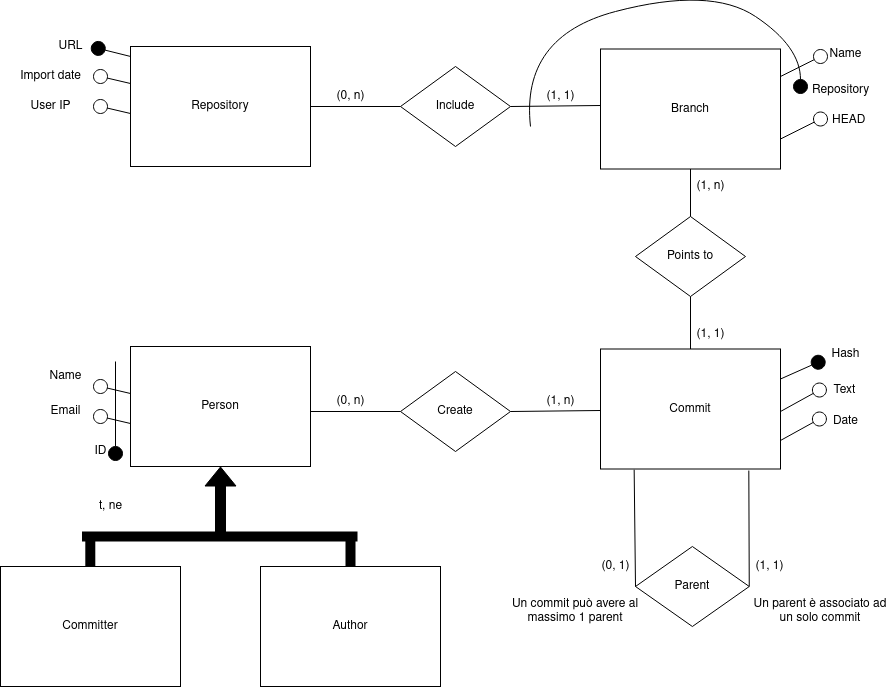
\includegraphics[scale=0.5]{data/er.png}
\caption{Modello E/R}
\label{}
\end{figure}

\chapter{Schema logico}
Qui di seguito è riportato uno schema logico del database mediante modello Relazionale.
\begin{figure}[htp]
\centering
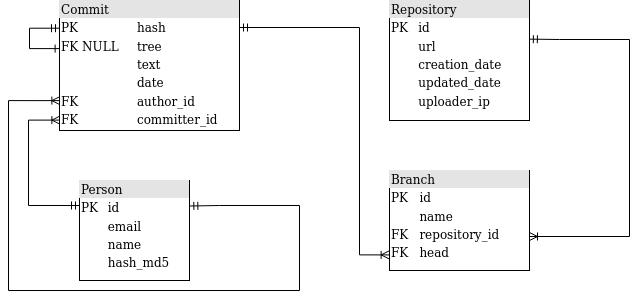
\includegraphics[scale=0.70]{data/relation.png}
\caption{Modello relazionale}
\label{}
\end{figure}

Come si può ben vedere sono state fatte delle modifiche:
\begin{itemize}
\item Repository: aggiunte le date di creazione e modifica;
\item Branch: ha un suo id come PK, in modo da accedervi più facilmente tramite backend. Questo perché i branch permettono anche lo slash nel nome, cosa che andrebbe a creare errore se passato nell'endpoint;
\item Commit: ha un campo \verb|tree| che si riferisce al parent: può ovviamente essere null. Dato che il commit può essere scritto da massimo 2 persone, ho preferito aggiungere i campi \verb|author_id| e \verb|commiter_id|;
\item Person: ha un campo \verb|hash_md5| che calcola l'MD5\footnote{https://en.wikipedia.org/wiki/MD5} dell'email una volta sola: usato per il gravatar;
\end{itemize}


\chapter{Schema fisico}
Qui di seguito è riportato il \verb|dump| in SQL per la creazione delle tabelle all'interno di PostgreSQL
\begin{lstlisting}[language=SQL]
CREATE TABLE "repository" (
    id serial PRIMARY KEY NOT NULL,
    url varchar(255) UNIQUE NOT NULL,
    created_date timestamp NOT NULL,
    updated_date timestamp NOT NULL,
	uploader_ip varchar(15) NOT NULL
);

CREATE TABLE "email"(
    email varchar(120) PRIMARY KEY NOT NULL,
    hash_md5 varchar(32) UNIQUE NOT NULL
);

CREATE TABLE "commit" (
    hash varchar(40) PRIMARY KEY NOT NULL,
    tree varchar(40) REFERENCES commit(hash) NULL,
    text text NOT NULL,
    date timestamp NOT NULL,
    author_email varchar(120) REFERENCES email(email) NOT NULL,
    author_name varchar(120) NOT NULL,
    committer_email varchar(120) REFERENCES email(email) NOT NULL,
    committer_name varchar(120) NOT NULL,
    repository_url varchar(256) REFERENCES repository(url) NOT NULL 
);

CREATE TABLE "branch" (
    id serial PRIMARY KEY NOT NULL,
    name varchar(120) NOT NULL,
    repository_id integer REFERENCES repository(id) NOT NULL,
    head varchar(40) REFERENCES commit(hash) NULL
);
\end{lstlisting}

\chapter{Conclusioni}
In conclusione posso dire che la webapp non è completa affatto. Come lei, qualsiasi altro software FOSS: esso può migliorare e mutare. Non posso dire con certezza che sarà mantenuto con costanza, ma ci proverò.


Una cosa che vorrei introdurre sono i \textit{commenti}: essi potranno riferirsi alla repository o al singolo commit.

Ci sono svariate altre modifiche per l'app backend e frontend che si potrebbero e dovrebbero fare, ma preferisco non includerle in questo documento. Ho citato prima i commenti perché sono una funzionalità lato backend che si interlacciano al database.\\\\
Il trigger mostrato nella \verb|Sezione 5.1| si riferisce al linguaggio SQL usato da PostgreSQL, lo si può reinterpretare senza la divisione con la procedura per dar luogo a un SQL più simile a quello visto durante il corso di Basi di Dati.\\\\
Le immagini sono state realizzate con un programma di terze parti\footnote{https://app.diagrams.net/}. Questo documento è stato realizzato in \LaTeX\ mediante Gummi\footnote{https://github.com/alexandervdm/gummi}.


\end{document}
